% !TEX root = ../thesis.tex

\newcommand{\fullyconnected}[1][]{
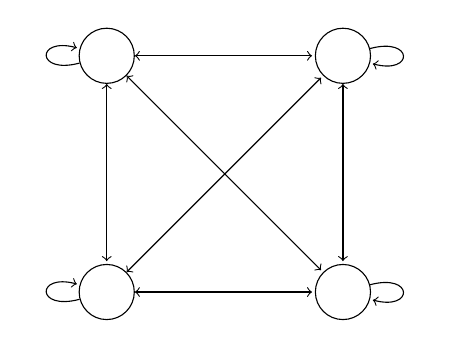
\begin{tikzpicture}[shorten >=1pt,<->,draw=black, node distance=\layersep]
	\tikzstyle{neuron}=[circle,draw=black,,minimum size=12pt,inner sep=0pt,text width=2em, text centered]    
	\node[neuron] (N-1) at (0,0) {};
	\node[neuron] (N-2) at (0,-3) {};
	\node[neuron] (N-3) at (3,0) {};
	\node[neuron] (N-4) at (3,-3) {};
	\path[] (N-1) edge [loop left] node {} (N-1);
	\path[] (N-2) edge [loop left] node {} (N-2);
	\path[] (N-3) edge [loop right] node {} (N-3);
	\path[] (N-4) edge [loop right] node {} (N-4);
         \path (N-1) edge (N-2);
         \path (N-1) edge (N-3);
         \path (N-1) edge (N-4);
          \path (N-2) edge (N-3);
          \path (N-2) edge (N-4);
          \path (N-3) edge (N-4);
\end{tikzpicture}
}
\newcommand{\partiallyconnected}[1][]{
\begin{tikzpicture}[shorten >=1pt,->,draw=black, node distance=\layersep]
	\tikzstyle{neuron}=[circle,draw=black,,minimum size=12pt,inner sep=0pt,text width=2em, text centered]    
	\node[neuron] (O-1) at (0,0) {};
	\node[neuron] (O-2) at (-4,0) {};
	\node[neuron] (H-1) at (0,-3) {};
	\node[neuron] (H-2) at (-4,-3) {};
	\node[neuron, label=below:C1] (I-1) at (-1,-6) {};
	\node[neuron, label=below:C2]  (I-2) at (1,-6) {};
	\node[neuron]  (I-3) at (-3,-6) {};
	\node[neuron] (I-4) at (-5,-6) {};
	
	\foreach \source in {1,2}{
		 \foreach \dest in {1,2} {
           		\path (H-\source.north) edge (O-\dest.south);
			\path (I-\source.north) edge (H-\dest.south);
		}
	}
	\foreach \source in {3,4}{
		 \foreach \dest in {1,2} {
			\path (I-\source.north) edge (H-\dest.south);
		}
	}
	\path[dashed] (H-1.north) edge[bend left=60] (I-2.east);
	\path[dashed] (H-2.north) edge[bend left=55]  ($(I-1.east)$);
\end{tikzpicture}

}